%%%%%%%%%%%%%%%%%%%%%%%%%%%%%%%%%%%%%%%%%%%%%%%%%%%%%%%%%%%%%%%%%%%%%%%%%%%%
% AGUtmpl.tex: this template file is for articles formatted with LaTeX2e,
% Modified March 2009
%
% This template includes commands and instructions
% given in the order necessary to produce a final output that will
% satisfy AGU requirements.
%
% PLEASE DO NOT USE YOUR OWN MACROS
%
% For more information on using the AGUTeX macro package,
% see agudocs.tex or agudocs.pdf
%
%%%%%%%%%%%%%%%%%%%%%%%%%%%%%%%%%%%%%%%%%%%%%%%%%%%%%%%%%%%%%%%%%%%%%%%%%%%%
%
% All questions should be e-mailed to author.help@agu.org.
%
%%%%%%%%%%%%%%%%%%%%%%%%%%%%%%%%%%%%%%%%%%%%%%%%%%%%%%%%%%%%%%%%%%%%%%%%%%%%
%
% Step 1: set the \documentclass
%
% The three options for article format are: two-column (default),
% draft, for initial article submission; and galley for narrow
% single columns.
%
% PLEASE USE THE DRAFT OPTION TO SUBMIT YOUR PAPERS
% The draft option produces double spaced output
%
% Choose the journal abbreviation for the journal you are
% submitting to:

% jgrga JOURNAL OF GEOPHYSICAL RESEARCH
% gbc   GLOBAL BIOCHEMICAL CYCLES
% grl   GEOPHYSICAL RESEARCH LETTERS
% pal   PALEOCEANOGRAPHY
% ras   RADIO SCIENCE
% rog   REVIEWS OF GEOPHYSICS
% tec   TECTONICS
% wrr   WATER RESOURCES RESEARCH
% gc    GEOCHEMISTRY, GEOPHYSICS, GEOSYSTEMS

% (If you are submitting to a journal other than jgrga,
% substitute the initials of the journal for "jgrga" below)

\documentclass[draft,grl]{agutex}

%%%%%%%%%%%%%%%%%%%%%%%%%%%%%%%%%%%%%%%%%%%%%%%%%%%%%%%%%%
%%%% optional article formats author might want to use

% To produce a galley version:
% \documentclass[galley,jgrga]{AGUTeX}

% To produce a two columned version:
% \documentclass[jgrga]{AGUTeX}

%%%%%%%%%%%%%%%%%%%%%%%%%%%%%%%%%%%%%%%%%%%%%%%%%%%%%%%%%%%%%%%%%%%%%%%%%
% OPTIONAL:
% To print your article using PostScript fonts, uncomment this:
% \usepackage{agu-ps}
% You many need to edit the top of agu-ps to use the names of the PS
% fonts on your system.

%%%%%%%%%%%%%%%%%%%%%%%%%%%%%%%%%%%%%%%%%%%%%%%%%%%%%%%%%%%%%%%%%%%%%%%%%
% OPTIONAL:
% To Create numbered lines:

% If you don't already have lineno.sty, you can download it from
% http://www.ctan.org/tex-archive/macros/latex/contrib/ednotes/
% (or google lineno.sty ctan), available at TeX Archive Network (CTAN).
% Take care that you always use the latest version.

% To activate the commands, uncomment \usepackage{lineno}
% and \linenumbers*[1]command, below:

\usepackage{lineno}
\linenumbers*[1]

%%%%%%%%%%%%%%%%%%%%%%%%%%%%%%%%%%%%%%%%%%%%%%%%%%%%%%%%%%%%%%%%%%%%%%%%%
% Figures and Tables
%

% When submitting articles through the GEMS system:
% COMMENT OUT ANY COMMANDS THAT INCLUDE GRAPHICS.
% (See FIGURES section near the end of the file)


%  Figures and Tables should be placed at the end of the article,
%  after the references.
%
%  Uncomment the following command to include .eps files
%  (comment out this line for draft format):
\usepackage[dvips]{graphicx}
%
%    Uncomment the following command to allow illustrations to print
%    when using Draft:
\setkeys{Gin}{draft=false}
%
% Substitute one of the following for [dvips] above
% if you are using a different driver program and want to
% proof your illustrations on your machine:
%
% [xdvi], [dvipdf], [dvipsone], [dviwindo], [emtex], [dviwin],
% [pctexps],  [pctexwin],  [pctexhp],  [pctex32], [truetex], [tcidvi],
% [oztex], [textures]
%
% See how to enter figures and tables at the end of the article, after
% references.
%
%% ------------------------------------------------------------------------ %%
%
%  ENTER PREAMBLE
%
%% ------------------------------------------------------------------------ %%

% Author names in capital letters:
\authorrunninghead{DAWE AND AUSTIN}

% Shorter version of title entered in capital letters:
\titlerunninghead{RECONCILING LES ENTRAINMENT}

% Author mailing address: please repeat this command for
% each author and alphabetize authors:

\authoraddr{Philip H. Austin,
Department of Earth and Ocean Sciences, University of
British Columbia, 6339 Stores Road, Vancouver, BC, V6T 1Z4, Canada.
(paustin@eos.ubc.ca)}

\authoraddr{Jordan T. Dawe,
Department of Earth and Ocean Sciences, University of
British Columbia, 6339 Stores Road, Vancouver, BC, V6T 1Z4, Canada.
(jdawe@eos.ubc.ca)}

\begin{document}

%% ------------------------------------------------------------------------ %%
%
%  TITLE
%
%% ------------------------------------------------------------------------ %%


\title{Reconciling direct and bulk tracer measurements of LES cloud entrainment}
%

%% ------------------------------------------------------------------------ %%
%
%  AUTHORS AND AFFILIATIONS
%
%% ------------------------------------------------------------------------ %%


%Use \author{\altaffilmark{}} and \altaffiltext{}

% \altaffilmark will produce footnote;
% matching altaffiltext will appear at bottom of page.
% May use \\ to start a new line.

\authors{Jordan T. Dawe\altaffilmark{1} and Philip H. Austin\altaffilmark{1}}

\altaffiltext{1}{Department of Earth and Ocean Sciences, 
                      University of British Columbia, Vancouver, BC, Canada}

%% ------------------------------------------------------------------------ %%
%
%  ABSTRACT
%
%% ------------------------------------------------------------------------ %%

% >> Do NOT include any \begin...\end commands within
% >> the body of the abstract.

\begin{abstract}
Direct measurements of entrainment and detrainment rates from LES model 
cloud fields produce values twice as large as those produced from bulk 
conserved tracer budget calculations.  This discrepancy is due to neglect of 
the influence of the moistened cloud environment on the tracer budget 
calculations.  Correcting the entrainment and detrainment values to account for 
the effect of the shell of moist air around the clouds corrects this 
over-estimate.  Estimates of effective entrainment and detrainment values for
specific humidity and liquid water moist static energy agree well with
conditional averages of cloud edge and shell values.  However, effective 
entrainment values of vertical velocity show marked differences from the 
vertical velocity present in the cloud shell.
\end{abstract}

%% ------------------------------------------------------------------------ %%
%
%  BEGIN ARTICLE
%
%% ------------------------------------------------------------------------ %%

% The body of the article must start with a \begin{article} command
%
% \end{article} must follow the references section, before the figures
%  and tables.

\begin{article}

%% ------------------------------------------------------------------------ %%
%
%  TEXT
%
%% ------------------------------------------------------------------------ %%

\section{Introduction}

The rate at which air is entrained into and detrained from clouds affects cloud 
properties, cloud top height, and vertical transports of heat and moisture.  
Proper simulation of these subgrid-scale effects in General Circulation Models 
(GCMs) therefore depends on accurate parameterization of entrainment and 
detrainment.

Large Eddy Simulation (LES) is a primary tool used to study these dynamics.  
LES entrainment and detrainment rates are typically calculated by recording 
budgets of bulk conserved tracer variables and inferring the amount of fluid 
exchange between the clouds and the surrounding air that is needed to balance 
vertical advection rates within the cloud field.  These rates are then used in 
simple entraining plume parameterizations to evaluate sub-grid scale cloud 
transports in GCMs.  \cite{Siebesma1995} derive the following equations for 
entrainment and detrainment from a simple entraining cloud core plume, where 
cloud core is defined as regions having condensed liquid water, positive 
buoyancy, and upward vertical velocity:
\begin{equation}
  \label{eq:siebesma_entrainment}
    E_{\phi}(\phi_c - \phi_e) = - M_c \frac{\partial \phi_c}{\partial z}
        - \frac{\partial \rho a \overline{w' \phi'}^c}{\partial z}
        - \rho a \frac{\partial \phi_c}{\partial t}
        + a \rho \left(\frac{\partial \bar{\phi}}{\partial t}\right)_{forcing}
\end{equation}
and
\begin{equation}
  \label{eq:siebesma_detrainment}
    D_{\phi}(\phi_c - \phi_e) = - M_c \frac{\partial \phi_e}{\partial z}
        + \frac{\partial \rho (1 - a) \overline{w' \phi'}^e}{\partial z}
        + \rho (1-a) \frac{\partial \phi_e}{\partial t}
     - \rho (1-a) \left(\frac{\partial \bar{\phi}}{\partial t}\right)_{forcing}
\end{equation}
Here $\phi$ represents any conserved bulk tracer, such as the total specific 
water $q_t$ (kg water kg$^{-1}$ moist air) or the liquid-water moist static 
energy $h$ (J kg$^{-1}$), $a$ is the fractional cloud core area, $\rho$ is the 
density of the air in kg m$^{-3}$, $M_c$ is vertical cloud core mass flux 
(kg m$^{-2}$ s$^{-1}$), $w$ is vertical velocity (m s$^{-1}$), $e$ and $c$ sub- 
and super-scripts denote horizontally averaged values conditionally sampled in 
the cloud environment and core, $forcing$ refers to forcings not included in 
the other terms, such as radiation or subsidence, primed values represent 
anomalies relative to the horizontal mean, overbars represent horizontal 
averaging, and $E_{\phi}$ and $D_{\phi}$ are the total bulk tracer entrainment 
into and detrainment out of the cloud core in kg s$^{-1}$ m$^{-3}$.  

Alternatively, entrainment and detrainment can be calculated directly from the 
LES velocity and tracer fields.  \cite{Romps2010} recently presented a 
technique to measure entrainment and detrainment in this manner.
\begin{equation}
  \label{eq:romps_e_minus_d}
  e - d = \frac{\partial}{\partial t}(\mathcal{A}\rho) 
        + \nabla \cdot (\rho \mathbf{u} \mathcal{A}) 
\end{equation}
Here $e$ and $d$ are the local entrainment and detrainment through the cloud 
surface in kg s$^{-1}$ m$^{-3}$, $\mathbf{u}$ is the velocity of the air in 
m s$^{-1}$, and $\mathcal{A}$ is the ``activity" of the fluid, where 
$\mathcal{A}$ is one at ``active" cloud core points and zero otherwise.  The 
values of $e - d$ are averaged over the length of time a grid cell experiences 
mass fluxes between an active and an inactive point, then positive $e-d$ values 
are considered to be purely $e$, and negative values, $d$.  Summing these point 
measurements horizontally allows one to calculate  $E_d$ and $D_d$, the total 
directly calculated cloud core entrainment and detrainment in kg s$^{-1}$ 
m$^{-3}$.

Romps found that direct measurement of the fluxes produced values roughly twice 
as large as tracer budget calculations.  Romps attributed this difference to 
the bulk tracer calculation assumption that the fluid exchanged between clouds 
and environment has the mean properties of the cloud or environment, 
respectively.  The unlikelyness of this assumption is suggested by recent 
studies of the dense, descending shell of moist air that forms around 
trade-wind cumulus clouds \citep{Heus2008, Wang2010}.  Since fluid exchanges 
between clouds and environment must pass through this shell, it is likely that 
it plays an important role in entrainment and detrainment dynamics.

Reconciling the direct flux and bulk tracer calculations is important if direct 
flux calculations are to be used to inform GCM parameteriztions.  Here we 
examine the sources of the factor of two discrepancy between the methods.  We 
show the discrepancy can be explained by three effects: the presence of the 
moist shell, Reynolds correlations between the entrainment rates and the tracer 
values, and numerical errors in the calculation methods.  We derive a 
correction to convert between ``tracer" and ``direct" entrainment fluxes, and 
then use this correction to evaluate the impact of variability in the moist 
shell on bulk tracer entrainment and detrainment rates.

%===================================================

\section{Model description}

All calculations in this paper were made using the System for Atmospheric 
Modeling \citep[SAM;][]{Khairoutdinov2003}.  Two model runs were performed, 
configured as standard Global Energy and Water Cycle Experiment (GEWEX) 
Cloud System Studies \citep[GCSS;][]{Randall2003} experiments: a Barbados 
Oceanographic and Meteorological Experiment \citep[BOMEX;][]{Siebesma2003} run,
and an Atmospheric Radiation Measurement Study \citep[ARM;][]{Brown2002} run. 
The BOMEX run was perfromed on a 6.4 km x 6.4 km horizontal x 3.2 km vertical 
domain with 25 meter grid resolution in all directions for 6 hours, and the 
first three hours of simulation were discarded. The ARM run was performed on a 
7.68 km x 7.68 km x 4.5 km domain with 30 meter grid resolution.

We have implemented the entrainment calculation scheme of \cite{Romps2010} in 
SAM, allowing us to calculate entrainment and detrainment directly from model 
mass fluxes.  These calculations were performed for fluxes into and out of the 
cloud core.  Romps also presents an equation for calculating tracer entrainment 
rates in the same framework, but neglects the effects of forcing and diffusion 
terms.  These terms are significant for tracer quantities like vertical 
momentum, so we include these effects in Romps's tracer equation:
\begin{equation}
  \label{eq:romps_ephi_minus_dphi}
  e\phi - d\phi = \frac{\partial}{\partial t}(\phi \mathcal{A} \rho) 
                + \nabla \cdot (\phi \rho \mathbf{u} \mathcal{A})
                - \mathcal{A}S_\phi
\end{equation}
where $S_\phi$ is any non-advective source term for $\phi$, in units of 
$[\phi]$ s$^{-1}$.  This equation is then averaged in the same way as equation 
(\ref{eq:romps_e_minus_d}), but since $\phi$ can be negative, negative 
entrainment fluxes are now possible.  If the average value of $\phi$ over the 
period of flux averaging is positive, then positive $e\phi-d\phi$ values are 
considered to be purely $e\phi$, and negative values, $d\phi$.  However, if 
$\phi$ is negative then positive $e\phi-d\phi$ values are considered to be 
purely $d\phi$, and negative values, $e\phi$.  Horizontal summation then gives 
$(E\phi)_d$ and $(D\phi)_d$, the total directly calculated tracer entrainment 
and detrainment for the cloud ensemble in $[\phi]$ kg s$^{-1}$ m$^{-3}$.

%===================================================

\section{The Cloud Shell}

The effective $q_t$ value of the entrained or detrained fluid can be easily 
calculated from the mass and tracer fluxes via $\phi_E = (E\phi)_d / E_d$ and 
$\phi_D = (D\phi)_d / D_d$, where $\phi_E$ and $\phi_D$ are the effective 
tracer values at which entrainment and detrainment occurs.  Examination of 
these values from the BOMEX model run shows significant differences between 
$q_E$ and the environmental $q_t$ and between $q_D$ and the core $q_t$ (Figure 
\ref{fig:Reynolds_correction}a), confirming that $q_E$ and $q_D$ do not occur 
at the mean environment and core values.  Near cloud base, $q_E$ and $q_D$ both 
have $q_t$ values matching the core.  They seperate within the cloud layer 
below the inversion, with $q_E$ values roughly halfway between the core and 
edge properties, and $q_D$ values halfway between $q_E$ and the core.  Near the 
inversion, $q_E$ and $q_D$ again become relatively more core-like as the 
environment rapidly dries.

Calculated ${q_t}_D$ values agree well with the mean ``cloud core edge" (cloud 
core model grid cells that are nearest-neighbour adjacent to non-core cells) 
$q_t$ values.  ${q_t}_E$ values, however, are moister than the mean ``cloud 
core shell" (non-core model grid cells that are nearest-neighbour adjacent to 
core cells) values.  This suggests that non-trivial Reynolds fluxes exist 
between $q_E$ and $e$: more entrainment occurs when $q_t$ is larger than the 
mean $q_t$ of the shell air, and less when $q_t$ is smaller.  This also implies 
shell dynamics have an active role in the tracer fluxes between cloud and 
environment.

%-------------------------------------------------------------------------

\subsection{$E$ and $D$ correction}
  
Here we derive a correction to equations (\ref{eq:siebesma_entrainment}) and 
(\ref{eq:siebesma_detrainment}) to account for the presence of the moist cloud 
shell and dry cloud edge, allowing us to convert between ($E_d, D_d$) and 
($E_\phi, D_\phi$).  We start our derivation by modifying equation (5.1) from
\cite{Siebesma1995}:
\begin{eqnarray}
  \label{eq:entrainment_derivation_1}
    \rho \frac{\partial a \phi_c}{\partial t} 
    = - \frac{\partial M_c \phi_c}{\partial z} 
    + E_d \phi_E - D_d \phi_D
    - \frac{\partial \rho a \overline{w' \phi'}^c}{\partial z} 
    + a \rho \left(\frac{\partial \bar{\phi}}{\partial t}\right)_{forcing}
\end{eqnarray}
\begin{eqnarray}
  \label{eq:detrainment_derivation_1}
    \rho \frac{\partial (1 - a) \phi_e}{\partial t}
    = \frac{\partial M_c \phi_e}{\partial z} 
    - E_d \phi_E + D_d \phi_D
    - \frac{\partial \rho (1 - a) \overline{w' \phi'}^e}{\partial z} 
    + \rho (1 - a) \left(\frac{\partial \bar{\phi}}{\partial t}\right)_{forcing}.
\end{eqnarray}
Here we have replaced $\phi_e$ in the entrainment term with $\phi_E$ and 
$\phi_c$ in the detrainment term with $\phi_D$, where $\phi_E$ and $\phi_D$ are 
the bulk tracer value of the air being entrained and detrained, respectively.

Next we substitute in the continuity equation for a cloud plume,
\begin{equation}
   \label{eq:continuity}
   \rho \frac{\partial a}{\partial t} 
   + \frac{\partial M_c}{\partial z} = E_d - D_d,
\end{equation}
allowing us to write
\begin{eqnarray}
  \label{eq:entrainment_derivation_2}
    E_d (\phi_c - \phi_E) - D_d (\phi_c - \phi_D)
    = M_c \frac{\partial \phi_c}{\partial z}
    + \frac{\partial \rho a \overline{w' \phi'}^c}{\partial z} 
    + \rho a \frac{\partial \phi_c}{\partial t}
    - a \rho \left(\frac{\partial \bar{\phi}}{\partial t}\right)_{forcing}
\end{eqnarray}
\begin{eqnarray}
  \label{eq:detrainment_derivation_2}
    D_d (\phi_e - \phi_D) + E_d (\phi_e - \phi_E)
    = M_c \frac{\partial \phi_e}{\partial z}
    - \frac{\partial \rho (1 - a) \overline{w' \phi'}^e}{\partial z} 
    - \rho (1 - a) \frac{\partial \phi_e}{\partial t}
    + \rho (1 - a) \left(\frac{\partial \bar{\phi}}{\partial t}\right)_{forcing}.
\end{eqnarray}

Finally, we substitute in equations (\ref{eq:siebesma_entrainment}) and 
(\ref{eq:siebesma_detrainment}) for the bulk tracer tendency terms and 
rearrange to get
\begin{equation}
  \label{eq:corrected_entrainment}
    E_{\phi} = E_d - E_d\frac{\phi_E - \phi_e}{\phi_{c} - \phi_{e}}
             - D_d\frac{\phi_c - \phi_D}{\phi_{c} - \phi_{e}}
\end{equation}
\begin{equation}
  \label{eq:corrected_detrainment}
    D_{\phi} = D_d - D_d\frac{\phi_c - \phi_D}{\phi_{c} - \phi_{e}}
             - E_d\frac{\phi_E - \phi_e}{\phi_{c} - \phi_{e}}.
\end{equation}
Note that under this correction $E_d-D_d = E_{\phi}-D_{\phi}$, preserving 
mass continuity.

Comparison of $E_{q_t}$ and $D_{q_t}$ ($E_{\phi}$ and $D_{\phi}$ inferred using 
specific humidity $q_t$ as the bulk tracer) with $E_d$ and $D_d$ calculated by 
the method of \cite{Romps2010} shows the directly calculated values are 
significantly larger than the bulk tracer values (Figure 
\ref{fig:Reynolds_correction}, b and c).  Correcting $E_d$ and $D_d$ using the 
mean $q_t$ of the cloud core edge and shell in place of $q_E$ and $q_D$ in 
equations (\ref{eq:corrected_entrainment}) and (\ref{eq:corrected_detrainment})
improves the agreement with the bulk tracer calculations.  Relative to the bulk 
tracer calculation, the corrected $E_{q_t}$ values are still too large near 
cloud base.  However, the correction does duplicate the negative $D_{q_t}$ 
values near cloud base that are typically produced by bulk tracer calculations.

Including the effect of Reynolds correlations by using $q_E = (E q_t)_d/E_d$ 
and $q_D = (D q_t)_d/D_d$ decreases the corrected $E_d$ and $D_d$ values even 
further (Figure \ref{fig:Reynolds_correction}, b and c).  This reduces the 
correction agreement with the bulk tracer calculation over most of the cloud 
layer, but also reduces the large entrainment values near cloudbase, improving 
the overall shape of the fluxes.  Still, the entrainment values corrected by 
$q_E$ and $q_D$ are about half the magnitude of the Siebesma bulk tracer 
values.

This overcorrection is the result of numerical errors due to the discrete 
grid on which the LES fluxes are calculated.  To show this, we use alternate 
alternative equations for the calculation of bulk tracer entrainment and 
detrainment, derived by \cite{Romps2010}:
\begin{equation}
  \label{eq:romps_bulk_entrainment}
    E_{\phi}(\phi_c - \phi_e) = \phi_c(E_d-D_d) - ((E\phi)_d - (D\phi)_d)
\end{equation}
\begin{equation}
  \label{eq:romps_bulk_detrainment}
    D_{\phi}(\phi_c - \phi_e) = \phi_e(E_d-D_d) - ((E\phi)_d - (D\phi)_d)
\end{equation}
Note that by substituting $(E\phi)_d = E_d \phi_E$ and $(D\phi)_d = D_d \phi_D$ 
into (\ref{eq:romps_bulk_entrainment}) and (\ref{eq:romps_bulk_detrainment}),
we can quickly recover (\ref{eq:corrected_entrainment}) and 
(\ref{eq:corrected_detrainment}).  Because of this, the Romps bulk tracer 
formulation agrees exactly with the result of the $q_E$ and $q_D$ correction,
producing smaller $E_{q_t}$ and $D_{q_t}$ values than the Siebesma bulk tracer 
calculation.  

Siebesma's bulk tracer calculation estimates vertical tracer fluxes from the 
mean profiles of tracer quantities, while Romps' calculation finds the flux for 
each grid cell directly from the numerical model's advection code.  Romps' 
calculation is therefore much more consistent with the model formulation than 
Siebesma's.  Conversely, Romps' calculation requires finding the difference of 
two large quantities ($\phi_c(E_d-D_d)$ and $(E\phi)_d - (D\phi)_d$), with all 
the problems that implies.  Both these calculation methods therefore are 
subject to numerical errors that reduce their accuracy.  

%------------------------------------------------------------------------------

\subsection{$h$, $w$, and Reynolds correlations}

Since Reynolds correlations between $e$ and $q_t$ appear to have an important 
effect on the measured moisture fluxes between cloud and environment, we now 
examine fluxes of heat, represented in SAM by the liquid water moist static 
energy $h$ (units of J kg$^{-1}$) or the vertical momentum, represeted in SAM 
by the vertical velocity $w$ (units of m s$^{-1}$).

$h$ shows a similar distribution of core, edge, shell, environment, $h_E$ and 
$h_D$ properties when compared to $q_t$, indicating a tight coupling between 
these variables in the cloud dynamics (Figure \ref{fig:profile_plots}a).  Near 
cloud base, edge, shell, $h_E$ and $h_D$ all converge on the core value, 
spreading out in the cloud layer and becoming relatively more core-like in the 
inversion.  $h_D$ is identical to the edge properties, while $h_D$ is smaller 
than $h$ in the shell, indicating the influence of Reynolds correlations 
between $e$ and $h$.

We can quantify the effect of these Reynolds correlations by looking at 
$A = (h_E - h_e)/(h_c - h_e)$ and $B = (h_c - h_D)/(h_c - h_e)$, the correction 
factors in equations (\ref{eq:corrected_entrainment}) and 
(\ref{eq:corrected_detrainment}).  Using the edge and shell values of $h$ for 
$h_E$ and $h_D$ shows $A$ to have a much larger effect than $B$, due to the 
larger difference between the shell and the environment than between the edge 
and the core.  $E_d$ is reduced by .2 by the $A$ correction, while .45 of
$D_d$ is removed by $B$.  If instead we use $h_E = (E h)_d/E_d$ and 
$h_D = (D h)_d/D_d$ in equations (\ref{eq:corrected_entrainment}) and 
(\ref{eq:corrected_detrainment}), $A$ is unchanged but $B$ increases to .6.  
Calculations for $q_t$ values show nearly identical results (not shown).

$w$ shows very different relative profiles compared to $q_t$ and $h$.  First, 
there is a much wider spread in the $w$ values, with the shell having nearly 
zero vertical velocity and the edge being halfway between the core and the 
environment.  $w_D$ is again similar to the value of $w$ in the edge, but $w_E$ 
is much larger than $w$ in the shell, and in fact is roughly the same value as 
$w_D$ over most of the cloud layer.  This strongly contradicts than the common 
assumptions that fluid entrained into the cloud core plume has zero or negative 
vertical momentum (*TK*).

These differences indicate that Reynolds correlations are much more important 
to the $w$ fluxes than the $q_t$ or $h$ fluxes.  Indeed, using the value 
of $w$ in the shell to calculate $A$ results in a value of only about .2, while
using $w_E$ increased $A$ to .45.  $B$ shows much less sensitivity to the 
Reynolds fluxes, but is still reduces by about .1 by substituting $w_D$ for the 
edge value of $w$.

%-------------------------------------------------------------------------

\subsection{Instantaneous Fields}

The source of these Reynolds fluxes, and the reason they affect $w$ more than 
$q_t$ or $h$, can be seen by comparing instantaneous snapshots of the model 
values $e$, $e_{q_t}$, and $e_w$.  Since \cite{Romps2010} method of calculating 
$e$ and $d$ requires long time averages over the period that the cloud surface
is adjacent to a grid cell, it is unfortunately unsuitable for calculating 
instantaneous fields.  Instead, we use an alternative method we have devised 
that substitutes spatial interpolation for time averaging \citep{Dawe2011}.  
This alternative method results in slightly smaller values of $e$ and $d$ than 
are produced by Romps' method, but the produced values show good agreement in 
variability. $eq_t$ and $ew$ are calculated simply by multiplying the value 
of $e$ by the values of $q_t$ and $w$, respectively.

Examination of these fields shows that, while $e$ and $eq_t$ have a very 
similar spatial pattern, $ew$ is concentrated in regions where strong updrafts 
are entering the cloud core (Figure \label{fig:w_entrainment_example}).  The 
reason for this can been seen by examining the buoyancy, condensed liquid water,
and vertical velocity fields that define the cloud core.  Of these three
fields, buoyancy is the strongest constraint on the core.  This results in 
areas far above cloud base where air has become negatively buoyant but 
maintains upward velocity and elevated moisture.  As this air continues to 
rise more condensation occurs, which heats the updraft, makes it positively 
buoyant, and thus entraining it into the core.  In this way, entrainment is 
positively correlated with both $q_t$ and $w$.  This process occurs fairly 
often in our model cloud field, as evidenced both by our manual examination of 
the output fields, and the size of the Reynolds flux terms in the mean 
profiles.

%-------------------------------------------------------------------------

\subsection{Shell Variability}

Finally we ask whether variability of the shell and edge properties has an 
impact on the measured variability in the bulk tracer calculations of $E$ and 
$D$.  To do this we turn to the ARM run, and simply look at the variability in 
$A = ({q_t}_c - {q_t}_E)/({q_t}_c - {q_t}_e)$ and 
$B = ({q_t}_D - {q_t}_e)/({q_t}_c - {q_t}_e)$.  These quantities indeed show 
strong variability over the ARM diurnal cycle (Figure 
\ref{fig:shell_variability}).  Near cloud base and within the inversion, $A$ 
is nearly one while $B$ is nearly zero.  As the clouds mix into the inversion 
over the course of the day, the values evolve until at mid-cloud layer, $A$ 
has values near .6 and $B$ near .2.  Performing this calculation with a fixed 
value of $({q_t}_c - {q_t}_e)$, to remove the possibility that these changes 
are simply due to movement of the mean environment and core profiles, shows 
similar results.  The shell is clearly an active player in the entrainment and 
detrainment fluxes.

%==============================================================================

\section{Discussion and Conclusion}

We have shown it is possible to explain the differences between entrainment and 
detrainment values calculated via bulk tracer budgets and direct flux 
calculations by taking into account the properties of the cloud shell, the 
effect of Reynolds correlations between fluxes and tracer values, and 
accuracy differences in the numerical methods used by the two calculations.
This suggests that the presence of the moist cloud shell, and indeed the 
variability within this shell, has a significant role in mediating fluxes 
between the clouds and the environment, and may be an important factor in 
improving parameterizations of shallow convection.

Significant Reynolds fluxes are apparent in tracer and vertical momentum 
entrainment fields.  These fluxes are the result of vertical advection of 
moist but negatively buoyant air into a region where condensation causes 
latent heating, making the air buoyant and entraining it into the core.
However, this process is not unique to the definition of cloud core.  Similar 
correlations appear when we perform these calculations for regions of
condensed liquid water, as vertical advection can drive cloud condensation and 
thus cause entrainment.

Whether one considers the bulk tracer or directly calculated flux values to be 
"correct" will depend on the purpose for which they are used.  The bulk tracer 
entrainment and detrainment values are well suited to calculating cloud moisture 
and energy fluxes in GCM sub-grid scale parameterizations, which only have 
access to large-scale mean bulk tracer values.  The influence of variability 
in the cloud shell would then simply be incorporated into the paramerizaiton 
of the bulk tracer entrainment and detrainment values.  On the other hand, 
direct fluxes may be needed for calculating fluxes of aerosols whose 
chemical properties are altered by reactions in the presence of liquid water 
\citep{Hoppel1994}.  

%%% End of body of article:

%%%%%%%%%%%%%%%%%%%%%%%%%%%%%%%%
%% Optional Appendix goes here
%
%%%%%%%%%%%%%%%%%
% Geophysical Research Letters only allows an appendix without a letter.
%% You can get this result with
%  \section*{Appendix}
%  or
%  \section*{Appendix: Title}
%%%%%%%%%%%%%%%%%
%
% \appendix resets counters and redefines section heads
% but doesn't print anything.
% After typing  \appendix
%
% \section{Here Is Appendix Title}
% will print
% Appendix A: Here Is Appendix Title
%
% \section*{Appendix}
% will print
% Appendix
%
% \section*{Appendix: Here Is Appendix Title}
% will print
% Appendix: Here Is Appendix Title
%
% For only 1 appendix \appendix \section{Appendix} is preferred.
% which will print
% Appendix A

%%%%%%%%%%%%%%%%%%%%%%%%%%%%%%%%%%%%%%%%%%%%%%%%%%%%%%%%%%%%%%%%
%
% Optional Glossary or Notation section, goes here
%
%%%%%%%%%%%%%%
% Glossary only allowed in Reviews of Geophysics
% \section*{Glossary}
% \paragraph{Term}
% Term Definition here
%
%%%%%%%%%%%%%%
% Notation -- End each entry with a period.
% \begin{notation}
% Term & definition.\\
% Second Term & second definition.
% \end{notation}
%%%%%%%%%%%%%%%%%%%%%%%%%%%%%%%%%%%%%%%%%%%%%%%%%%%%%%%%%%%%%%%%
%
%  ACKNOWLEDGMENTS

\begin{acknowledgments}
Support for this work was provided by the Canadian Foundation for Climate and 
Atmospheric Science through the Cloud Aerosol Feedback and Climate network.
We thank Marat Khairoutdinov for making SAM available to the cloud modeling 
community.  All figures were generated using the matplotlib library in the 
Python programming language.
\end{acknowledgments}

%% ------------------------------------------------------------------------ %%
%
%  REFERENCE LIST AND TEXT CITATIONS
%
% Either type in your references using
% \begin{thebibliography}{}
% \bibitem{}
% Text
% \end{thebibliography}
%
% Or,
%
% If you use BiBTeX for your References, please produce your .bbl
% file and copy the contents into your paper here.
%
% Follow these steps:
% 1. Run LaTeX on your LaTeX file.
%
% 2. Run BiBTeX on your LaTeX file.
%
% 3. Open the new .bbl file containing the reference list and
%   copy all the contents into your LaTeX file here.
%
% 4. Comment out the old \bibliographystyle and \bibliography commands.
%
% 5. Run LaTeX on your new file before submitting.
%
% AGU does not want a .bib or a .bbl file, but asks that you
% copy in the contents of your .bbl file here.


%\begin{thebibliography}{}

\bibliography{shell_correction}
\bibliographystyle{agu}

%\bibitem[{\textit{Kilby}(2008)}]{jskilby}
%Kilby, J. S. (2008), Invention of the integrated circuit, {\it IEEE
%Trans. Electron Devices,} \textit{23}, 648--650.

%\bibitem[{\textit{Kilby et al.}(2008)}]{jskilbye}
%Kilby, J. S., S. Smith, and R. Jones (2008), Invention of the
%integrated circuit, {\it IEEE Trans. Electron Devices,} \textit{23},
%648--650.

%\end{thebibliography}

%Reference citation examples:

%...as shown by \textit{Kilby} [2008].
%...has been shown [\textit{Kilby et al.}, 2008].

%...as shown by \cite{jskilby}.
%...has been shown \citep{jskilbye}.


%% ------------------------------------------------------------------------ %%
%
%  END ARTICLE
%
%% ------------------------------------------------------------------------ %%

\end{article}

%% Enter Figures and Tables here:

% When submitting articles through the GEMS system:
% COMMENT OUT ANY COMMANDS THAT INCLUDE GRAPHICS.

% Figure captions go below this illustration; Table captions go above tables

\begin{figure}
  \noindent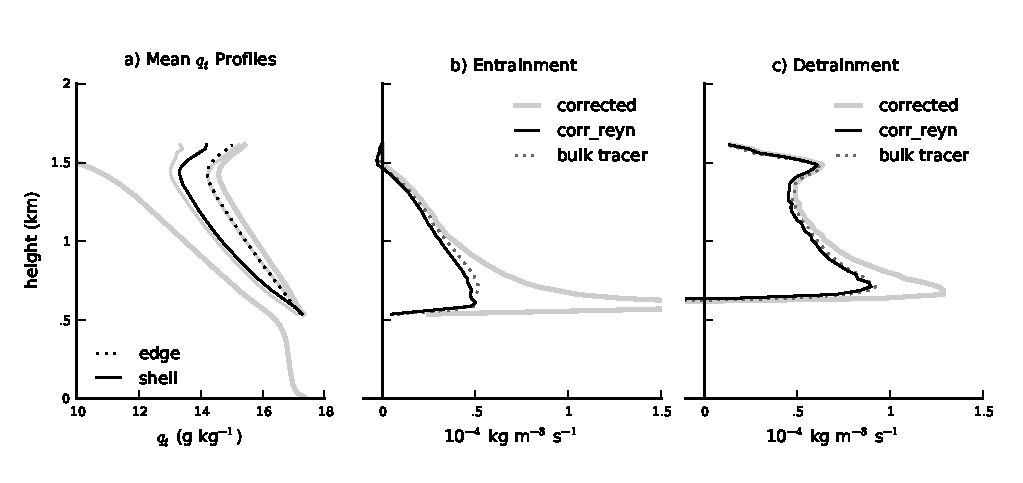
\includegraphics[width=39pc]{./figures/reynolds_correction}
  \caption{Result of correcting direct entrainment values for the presence of 
  the moist cloud shell.  a) Mean profiles of the effective total specific 
  water values being entrained ($q_E$, black line), and detrained ($q_D$ dotted 
  line), overlaid on the total specific water in the cloud core (thick dark 
  grey line), cloud core edge (thin dark grey line), cloud core shell (thin 
  grey line), and cloud core environemnt (thick grey line).  These $q_t$ values 
  are used to correct values of b) entrainment and c) detrainment; shown are the 
  direct flux calculation of \cite{Romps2010} (thick grey line), the bulk 
  tracer budget calculation of \cite{Siebesma1995} (dotted line), the direct 
  flux calculation corrected by the mean core shell and edge values (thin grey 
  line), and the direct flux calculation corrected by the $q_E$ and $q_D$ 
  values (black line).}
  \label{fig:Reynolds_correction}
\end{figure}

\begin{figure}
  \noindent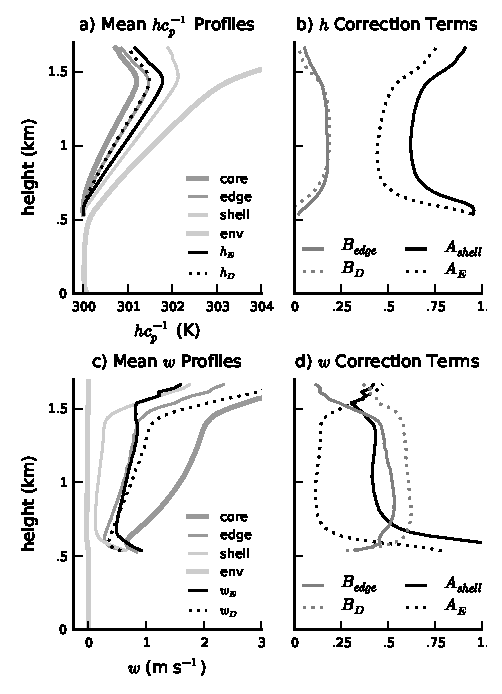
\includegraphics[width=20pc]{./figures/profile_plots}
  \caption{Mean profiles of a) liquid-water moist static energy values for 
  entraining (black line) and detraining (dotted line) air, overlaid on the 
  mean core, edge, shell, and environment profiles (grey lines), and b) the 
  resulting $(h_E - h_e)/(h_c - h_e)$ and $(h_c - h_D)/(h_c - h_e)$ profiles.  
  c) and d) are the same as a) and b), but calculated for $w$. 
}
  \label{fig:profile_plots}
\end{figure}

\begin{figure}
  \noindent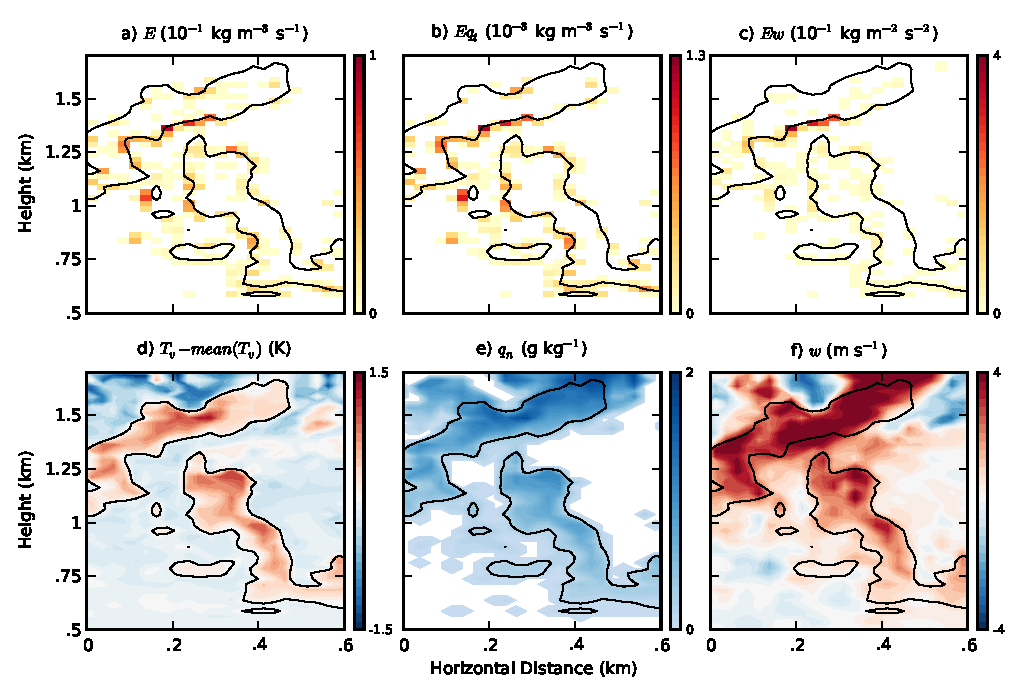
\includegraphics[width=39pc]{./figures/w_entrainment_example}
  \caption{Instantaneous vertical cross-section of cloud core mass entrainment 
  (a), humidity entrainment (b), vertical velocity entrainment (c), buoyancy 
  (d), condensed liquid water (e), and vertical velocity (f) of a single model
  cloud, illustrating the Reynolds correlation between vertical velocity and 
  entrainment.  Black lines indicate the edge of the cloud core in each figure.}
  \label{fig:w_entrainment_example}
\end{figure}


\begin{figure}
  \noindent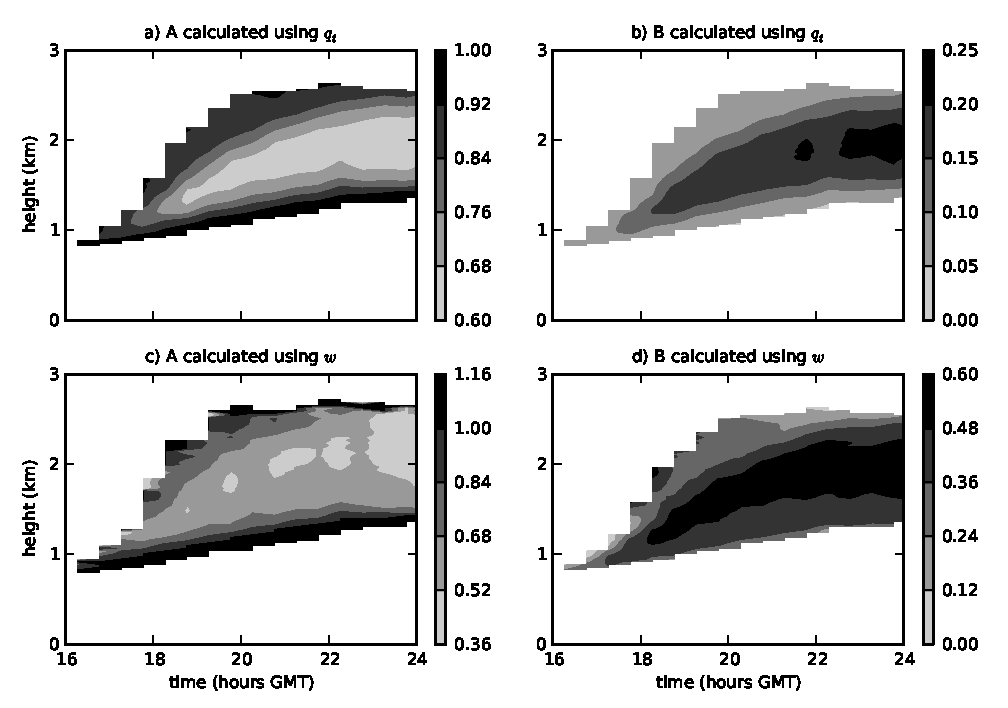
\includegraphics[width=20pc]{./figures/shell_variability}
  \caption{Variation in a) $({q_t}_E - {q_t}_e)/({q_t}_c - {q_t}_e)$ and b)
  $({q_t}_c - {q_t}_D)/({q_t}_c - {q_t}_e)$ over the duration of the ARM model run.
  }
  \label{fig:shell_variability}
\end{figure}

% ONE-COLUMN figure/table, including eps graphics
%
% \begin{figure}
% \noindent\includegraphics[width=20pc]{samplefigure.eps}
% \caption{Caption text here}
% \end{figure}
% \end{document}
%
% \begin{table}
% \caption{}
% \end{table}
%
% ---------------
% TWO-COLUMN figure/table
%
% \begin{figure*}
% \noindent\includegraphics[width=39pc]{samplefigure.eps}
% \caption{Caption text here}
% \end{figure*}
%
% \begin{table*}
% \caption{Caption text here}
% \end{table*}
%
% see below for how to make landscape figures or tables

%%% End the article here:

\end{document}

%%%%%%%%%%%%%%%%%%%%%%%%%%%%%%%%%%%%%%%%%%%%%%%%%%%%%%%%%%%%%%%


%% ------------------------------------------------------------------------ %%
%
%  IN-TEXT LISTS
%
%% ------------------------------------------------------------------------ %%

% Do not use bulleted lists; enumerated lists are okay.
% \begin{enumerate}
% \item
% \item
% \item
% \end{enumerate}

%% ------------------------------------------------------------------------ %%
%
%  EQUATIONS
%
%% ------------------------------------------------------------------------ %%

% Single-line equations are centered.

% Math coded inside display math mode \[ ...\]
% will not be numbered e.g.:
% \[ x^2=y^2 + z^2\]

% Math coded inside \begin{equation} and \end{equation} will
% be automatically numbered e.g.:
% \begin{equation}
% x^2=y^2 + z^2
% \end{equation}

% IF YOU HAVE MULTI-LINE EQUATIONS, PLEASE
% BREAK THE EQUATIONS INTO TWO OR MORE LINES
% OF SINGLE COLUMN WIDTH (20 pc, 8.3 cm)
% using double backslashes (\\).

% To create multiline equations, use the
% \begin{eqnarray} and \end{eqnarray} environment
% as demonstrated below.
\begin{eqnarray}
  x_{1} & = & (x - x_{0}) \cos \Theta \nonumber \\
        && + (y - y_{0}) \sin \Theta  \nonumber \\
  y_{1} & = & -(x - x_{0}) \sin \Theta \nonumber \\
        && + (y - y_{0}) \cos \Theta.
\end{eqnarray}

If you don't want an equation number, use the star form:
\begin{eqnarray*}...\end{eqnarray*}

% Break each line at a sign of operation
% (+, -, etc.) if possible, with the sign of operation
% on the new line.

% Indent second and subsequent lines to align with
% the first character following the equal sign on the
% first line.

% Use an \hspace{} command to insert horizontal space
% into your equation if necessary. Place an appropriate
% unit of measure between the curly braces, e.g.
% \hspace{1in}; you may have to experiment to achieve
% the correct amount of space.

% There is another multiline equation environment:
% \begin{aguleftmath}...\end{aguleftmath}
% The equation is aligned left and the second line indents to
% the width of a paragraph indent (AGU style)


%% ------------------------------------------------------------------------ %%
%
%  EQUATION NUMBERING: COUNTER
%
%% ------------------------------------------------------------------------ %%

% You may change equation numbering by resetting
% the equation counter or by explicitly numbering
% an equation.

% To explicitly number an equation, type \eqnum{}
% (with the desired number between the brackets)
% after the \begin{equation} or \begin{eqnarray}
% command.  The \eqnum{} command will affect only
% the equation it appears with; LaTeX will number
% any equations appearing later in the manuscript
% according to the equation counter.
%
% To reset the equation counter, place the setcounter{equation}
% command in front of your equation(s).
%\setcounter{equation}{0}

% Set the equation counter to 0 if the next
% number needed is 1 or set it to 7 if the
% next number needed is 8, etc.
%
% The \setcounter{equation} command does affect
% equations appearing later in the manuscript.

% If you have a multiline equation that needs only
% one equation number, use a \nonumber command in
% front of the double backslashes (\\) as shown in
% the multiline equation above.



%%%%%%%%%%%%%%%%%%%%%%%%%%%%%%%%%%%%%%%%%%%%%%%%%%%%%%
%% Landscape figure and table examples
%
% ---------------
% Landscape (broadside) figure/table
% (These objects will not display properly in draft mode, use galley.)
%
% ONE-COLUMN landscape figure and table
%
% \begin{landscapefigure}
% \includegraphics[height=.75\mycolumnwidth,width=42pc]{samplefigure.eps}
% \caption{Caption text here}
% \end{landscapefigure}
%
% \begin{landscapetable}
% \caption{Caption text here}
% \begin{tabular*}{\hsize}{@{\extracolsep{\fill}}lcccc}
% \tableline
% ....
% \tableline\\
% \multicolumn5l{(a) Algorithms from Numerical Recipes}\\
% \end{tabular*}
% \tablenotetext{}{}
% \tablecomments{}
% \end{landscapetable}
%
% FULL-PAGE landscape figures and tables
%
% \begin{figure*}[p]
% \begin{landscapefigure*}
% illustration here
% \caption{caption here}
% \end{landscapefigure*}
% \end{figure*}
%
% \begin{table}[p]
% \begin{landscapetable*}
% \caption{}
% \begin{tabular*}{\textheight}{@{\extracolsep{\fill}}lccrrrcrrr}
% ....
% \end{tabular*}
% \begin{tablenotes}
% ...
% \end{tablenotes}
% \end{landscapetable*}
% \end{table}
%
